%================================================================
\chapter{Quantum Computing}\label{chap:QuantumComputing}
%================================================================
This chapter introduces the fundamentals of quantum computing. The content of this chapter is mainly based on material in \citet{NielsenQuantum}.


%================================================================
\section{States in Quantum Mechanics}\label{sec:IntroQM}
%===============================================================
In quantum mechanics, isolated physical systems are completely described by its \emph{state vector}, which lives in a complex vector space. In this thesis, we will focus on finite vector spaces $\mathbb{C}^n$, where states are n-tuples of complex numbers $(z_1, \cdots, z_n)$ called \emph{amplitudes}. Adopting Dirac notation, a state is denoted as 
\begin{equation}
    \ket{\psi} \sim \begin{bmatrix}
           z_{1} \\
           \vdots \\
           z_{n}
         \end{bmatrix},
\end{equation}
where $\psi$ is the label of the state, and $\ket{\cdot}$ indicates that it is a vector. More specifically, in quantum mechanics, the states live in \emph{Hilbert spaces}, which is a vector space that has a well-defined inner product. The inner product of two states $\ket{\psi}, \ket{\psi'} \in \mathbb{C}^n$ is denoted 

\begin{equation}
    \braket{\psi'}{\psi} \equiv [z_1'^*, \cdots, z_n'^*] 
    \begin{bmatrix}
        z_{1} \\
        \vdots \\
        z_{n}
    \end{bmatrix}
    = \sum_{i=1}^{n} z_i'^* z_i, 
\end{equation}
where $z^*$ indicates the complex conjugate, i.e. if $z = a + ib$, we have that $z^* = a - ib$. As a constraint on the amplitudes, state vectors describing physical systems unit norm, meaning 

\begin{equation}
    \braket{\psi}{\psi} \equiv [z_1^*, \cdots, z_n^*] 
    \begin{bmatrix}
        z_{1} \\
        \vdots \\
        z_{n}
    \end{bmatrix}
    = \sum_{i=1}^{n} |z_i|^2 = 1.
\end{equation}

%================================================================
\subsection{The Qubit}\label{sec:TheQubit}
%===============================================================
As is common in quantum computing, we will be focusing on perhaps the simplest possible quantum system, the \emph{qubit}, which is a two-level system defined on $\mathbb{C}^2$.  There are multiple ways of implementing qubits in hardware, some of which will be discussed later, although  the specific physical realization is not necessary to account for when discussing quantum computing. In abstract terms, the state of a qubit can be formulated as

\begin{equation}
\ket{\psi} = \alpha \ket{0} + \beta \ket{1},
\end{equation}
where $\alpha$ and $\beta$ are complex numbers, and $\ket{0}$ and $\ket{1}$ are orthonormal states known as the \emph{computational basis states} and are specially defined by the implementation of the hardware. This linear combination of states is an important principle of quantum mechanics and is called \emph{superposition}; the system is in neither state $\ket{0}$ nor $\ket{1}$, but both at the same time(unless either $\alpha$ or $\beta$ is zero). In general, if states $\ket{\psi}$ and $\ket{\phi}$ are allowed, then so is the linear combination $\alpha \ket{\psi} + \beta \ket{\phi}$, where $|\alpha|^2 + |\beta|^2 = 1$.

Being the "atom" of quantum computing, the qubit is very reminiscent of the classical bit, which is always definitely "0" or "1". However, as we have seen, the qubit also may assume any normalized linear combination of the two states.
%================================================================
\subsection{Multiple Qubits}\label{sec:Multiple Qubits}
%===============================================================
As a central property of quantum mechanics, it is possible to create composit systems by combining several smaller quantum systems. This can be used to construct systems of multiple qubits, whose state can be expressed, if the qubits are independent, as

\begin{equation}\label{eq:tensorProductState}
\ket{\psi_1 \psi_2 \cdots \psi_n} \equiv \ket{\psi_1} \otimes \ket{\psi_2} \otimes \cdots \ket{\psi_n}.
\end{equation}
Here, the tensor product "$\otimes$" was used to indicate that each state $\ket{\psi_i}$ lives in its own $\mathbb{C}^2$ space. Using the principle of superpostion, one may make a linear combination of several multi-qubit states, where each $\ket{\psi_i}$ is either $\ket{0}$ or $\ket{1}$. In general, this can be written as

\begin{equation}\label{eq:MultiQubitState}
\ket{\psi} = \sum_{\boldsymbol{v}}c_{\boldsymbol{v}}\ket{\boldsymbol{v}_1} \otimes \ket{\boldsymbol{v}_2} \otimes \cdots \ket{\boldsymbol{v}_n},
\end{equation}
where $\boldsymbol{v} \in \{0,1\}^n$ sums over all possible binary strings of length $n$. As there are $2^n$ unique strings, we arrive at the remarkable result that one also needs $2^n$ amplitudes $c_{\boldsymbol{v}}$ to describe the state of $n$ qubits in general. In other words, the information stored in the quantum state of $n$ qubits in exponential in $n$, as opposed to the linear information of a equivalent classical system of classical bits. In a sense, the quantum information is "larger" than the classical information. This is a fascinating property of the  capabilities of quantum computing, which we will return to when discussing the usefulness of quantum computing in relation to machine learning.

%================================================================
\subsection{Measuring Qubits}\label{sec:MeasuringState}
%===============================================================
It appears the information encoded in quantum systems is much greater than the information in a corresponding classical system, at least in the case of qubits versus bits. How can one interact with this information? Unlike classical bits, whose state can always be measured exactly, the state of one or multiple qubits can not be measured and determined. Returning to the single qubit example, one can choose to perform a measurement in the computational basis on a qubit in the state $\ket{\psi} = \alpha \ket{0} + \beta \ket{1}$. The measurement will result in  \emph{either} $\ket{0}$ \emph{or} $\ket{1}$, with probability $|\alpha|^2$ and $|\beta|^2$, respectively. For multiple qubits in a general state \autoref{eq:MultiQubitState}, a measurement on all qubits will grant a state in the computational basis, i.e. $\ket{\boldsymbol{v}_1} \otimes \ket{\boldsymbol{v}_2} \otimes \cdots \ket{\boldsymbol{v}_n}$ for some binary string $\boldsymbol{v} \in \{0,1\}^n$, with probability $|c_{\boldsymbol{v}}|^2$. This motivates why states in quantum mechanics needs to have unity norm, i.e
\begin{equation}\label{eq:MultiQubitState}
\sum_{\boldsymbol{v}}|c_{\boldsymbol{v}}|^2 = 1,
\end{equation} 
as the probabilities of any outcome must sum to $1$.

%================================================================
\section{Quantum Circuits}\label{sec:QuantumCircuits}
%===============================================================
We have until now looked into how quantum states can encode information, and how information can be interacted with via measurement. How then can quantum mechanics be used for computation? To do computations, it is necessary to introduce some dynamical transformation of the quantum state. In quantum mechanics, transformations can be formulated as 

\begin{equation}\label{eq:UnitaryEvolution}
 \ket{\phi} = U\ket{\psi},
\end{equation}
where $U$ is a \emph{unitary} operator that acts on the vector space where $\ket{\psi}$ and $\ket{\phi}$ lives. Unitary means that the operator $U$ is linear with the property that $U^{\dagger} = U^{-1}$, that is, the Hermitian conjugate is equal to its inverse. This is a necessary property of linear operators in quantum mechanics as to ensure that the state stays normalized to 1:

\begin{equation}\label{eq:UnitaryEvolution}
 \braket{\phi}{\phi} = \bra{\psi}\underset{I}{\underbrace{U^{\dagger}U}}\ket{\psi} = \bra{\psi}\ket{\psi} =1.
\end{equation}
Assuming $\ket{\psi}$ is initially normalized, so is $\ket{\phi}$ after a unitary transformation.

By construction, quantum computers allow for the application of carefully selected sequences of operators that transforms the state in a desired way, often called a \emph{quantum circuit}. Typical operators used in quantum computing, often called quantum gates, act on either on one or multiple qubits, and bear resemblance to logical operations in the classical context. 

\autoref{fig:exampleCircuit} illustrates an example of a quantum circuit. Going from left to right indicates the chronological order of application of the different quantum gates. Note that the exact passing of time is not seen in this schematic, and is highly dependent on the implementation of physical hardware. The horizontal lines, called wires, each symbolize a qubit. From the notation on the left hand, it can be seen that all qubits are initialized in the zero state. Then, various gates are applied to the qubits, acting on one, two or three qubits. Lastly, illustrated by the gauge symbol, each qubit is measured in the computational basis, yielding either $0$ or $1$. This information is then stored in the classical register $c$, indicated by the double line. 

\begin{figure}[htp]
    \centering
    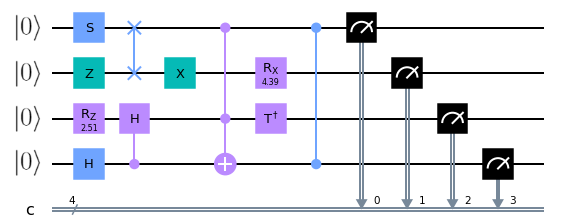
\includegraphics[width=10cm]{latex/figures/example_circuit.png}
    \caption{Example circuit consisting of 4 qubits initialized to $\ket{0}$. A random selection of quantum gates acting on one, two and three qubits are then applied. Finally, all qubits are measured in the computational basis and stored in a classical register.}
    \label{fig:exampleCircuit}
\end{figure}

%================================================================
\subsection{Single Qubit Operations}\label{sec:ControlledOperations}
%===============================================================

Returning again to the single qubit, the state of a qubit can be represented as a vector
\begin{equation}\label{eq:vectorRepresentation}
\ket{\psi} = \alpha \ket{0} + \beta \ket{1} \equiv \alpha 
    \begin{bmatrix}
        1 \\
        0
    \end{bmatrix} + 
    \beta \begin{bmatrix}
        0 \\
        1
    \end{bmatrix}
    =
    \begin{bmatrix}
        \alpha \\
        \beta
    \end{bmatrix}.
\end{equation}
Likewise, linear operators acting on a single qubit can in general be represented by a $2\times 2$ matrix 
\begin{equation}\label{eq:matrixRepresentation}
    \begin{bmatrix}
        c_{11} & c_{12} \\
        c_{21} & c_{22}
    \end{bmatrix},
\end{equation}
which is unitary. A highly interesting single qubit quantum gate is the Hadamard gate, which is formulated as 

\begin{equation}\label{eq:matrixRepresentation}
    H = \frac{1}{\sqrt{2}}\begin{bmatrix}
        1 & 1 \\
        1 & -1
    \end{bmatrix} = 
    \Qcircuit @C=1em @R=.7em {& \gate{H} & \qw}\\.
\end{equation}
Acting on the computational basis, the Hadamard gate can be seen to produce super positions
\begin{align*}
    H\ket{0} = \frac{1}{\sqrt{2}}\ket{0} +\frac{1}{\sqrt{2}}\ket{1}\\
    H\ket{1} = \frac{1}{\sqrt{2}}\ket{0} -\frac{1}{\sqrt{2}}\ket{1},
\end{align*}
which will lead to a $50\%$ chance to yield either $0$ or $1$ upon measuring. In a sense, this is the quantum mechanical equivalent to a coin toss. However, it is actually much more interesting. If applied a second time, we actually return to the original state, "unscrambling" the coin, or qubit:

\begin{equation}\label{eq:unscramble}
    HH\ket{0} = \frac{1}{\sqrt{2}}H\ket{0} +\frac{1}{\sqrt{2}}H\ket{1} = \frac{1}{2}(\ket{0} + \ket{0}) + \frac{1}{2}(\ket{1} - \ket{1}) = \ket{0}.
\end{equation}
Pointed out in \citet{SupervisedwquantumComputers}, this has no classical equivalent. If one has a classical procedure of scrambling a coin, e.g. shaking it in your hands, a second shaking will not leave it unscrambled, but scrambled still. Quantum computation is able to reverse this because quantum mechanics is fundamentally not a theory of probabilities; Probabilities can be derived from the theory, but the underlying description revolves around amplitudes, as explained earlier. Whereas probabilities must be positive or zero, amplitudes can be positive or negative(and complex in general), allowing for destructive interference. This can be seen in \autoref{eq:unscramble}, where the last term $\frac{1}{2}(\ket{1} - \ket{1})$ is cancelled out. In addition to the exponential large size of Hilbert space, this is also an interesting property of quantum computing when discussing its capabilities over classical computing.

Further, a much-used set of single qubit gates are the Pauli operators:

\begin{equation}
\begin{aligned}
    X = \sigma_x = 
    \begin{bmatrix}
        0 & 1 \\
        1 & 0
    \end{bmatrix} = 
    \Qcircuit @C=1em @R=.7em {& \gate{X} & \qw}\\
    Y = \sigma_y = 
    \begin{bmatrix}
        0 & -i \\
        i & 0
    \end{bmatrix} = 
    \Qcircuit @C=1em @R=.7em {& \gate{Y} & \qw}\\
    Z = \sigma_z = 
    \begin{bmatrix}
        1 & 0 \\
        0 & -1
    \end{bmatrix} = 
    \Qcircuit @C=1em @R=.7em {& \gate{Z} & \qw}
\end{aligned}    
\end{equation}

To visualize what these operators do, it is useful to introduce a graphical picture called the \emph{Bloch sphere}, illustrated in \autoref{fig:blochsphere}. Rewriting the state of a qubit to 

\begin{equation}\label{eq:blochsphere}
    \ket{\psi} = \alpha \ket{0} + \beta \ket{1} = e^{i\gamma}(\cos{\frac{\theta}{2}}\ket{0} + e^{i\phi}\sin{\frac{\theta}{2}}\ket{1}) \sim 
    \cos{\frac{\theta}{2}}\ket{0} + e^{i\phi}\sin{\frac{\theta}{2}}\ket{1},
\end{equation}
the new parameters $\theta$ and $\phi$ can be identified as the azimuthal and polar angles, respectively. Here, the factor $e^{i\gamma}$ is known as a global phase, which is not physically important to include. Using this, any single qubit state can then be identified as a point on the Bloch sphere.

\begin{figure}[htp]
    \centering
    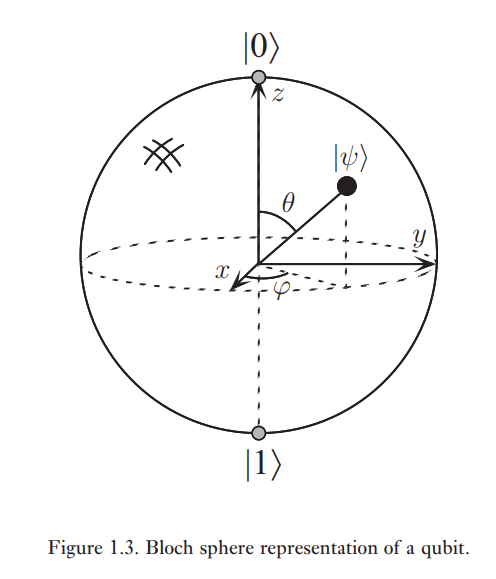
\includegraphics[width=10cm]{latex/figures/Blochsphere.PNG}
    \caption{Graphical picture visualizing the state of a qubit, called the Bloch sphere. The figure is retrived from \cite{NielsenQuantum}.}
    \label{fig:blochsphere}
\end{figure}

The Pauli-gates represent $180^{\circ}$ rotation of the state around the corresponding axis. Particlularly, the $X$ gate, often called the \emph{flip gate}, acts on the basis states as

\begin{equation}
\begin{aligned}
    X\ket{0} = \ket{1} \\
    X\ket{1} = \ket{0} \\
    X(\alpha \ket{0} + \beta\ket{1}) = \beta \ket{0} + \alpha\ket{1}.
\end{aligned}    
\end{equation}
Much like how the classical NOT-gate flips the bit, the X gate flips the qubit.

Another set of gates extremely important for quantum machine learning, which can be derived from the aforementioned Pauli gates, are the \emph{Pauli rotations}. They are formulated as exponentiated Pauli gates in the following way:

\begin{equation}\label{eq:PauliRotations}
\begin{aligned}
    R_x(\theta) = e^{-i\theta\sigma_x/2} = \cos{\frac{\theta}{2}}I - i\sin{\frac{\theta}{2}}\sigma_x
    =
    \begin{bmatrix}
        \cos{\frac{\theta}{2}} & -i\sin{\frac{\theta}{2}} \\
        -i\sin{\frac{\theta}{2}} & \cos{\frac{\theta}{2}}
    \end{bmatrix}\\
    R_y(\theta) = e^{-i\theta\sigma_y/2} = \cos{\frac{\theta}{2}}I - i\sin{\frac{\theta}{2}}\sigma_y
    =
    \begin{bmatrix}
        \cos{\frac{\theta}{2}} & -\sin{\frac{\theta}{2}} \\
        \sin{\frac{\theta}{2}} & \cos{\frac{\theta}{2}}
    \end{bmatrix}\\
    R_z(\theta) = e^{-i\theta\sigma_z/2} = \cos{\frac{\theta}{2}}I - i\sin{\frac{\theta}{2}}\sigma_z
    =
    \begin{bmatrix}
        e^{-i\theta/2} & 0 \\
        0 & e^{i\theta/2}
    \end{bmatrix}\\.
\end{aligned}    
\end{equation}

These action of these gates on any state is to rotate it on the Bloch sphere around the corresponding axis, for an amount of $\theta$ radians. As $\theta$ can be any real number, these gates can be though of as being quantum gates parameterized by $\theta$, which will be an essential component when we will construct \emph{parameterized quantum circuits} later.  









%================================================================
\subsection{Controlled Operations}\label{sec:ControlledOperations}
%===============================================================
With only single qubit gates, the number of states we can access is greatly reduced as all the qubits stay independent, i.e. the state can be written as \autoref{eq:tensorProductState}. By introducing gates that operates on several qubits, one can for example transform the state of one qubit conditioned on the state of an other qubit. This makes the two qubits correlated, known as \emph{entanglement} in quantum mechanics.

One such conditional gate is the controlled NOT gate(CNOT gate). It is formulated as

\begin{equation}
    CNOT = 
    \ket{0}\bra{0}\otimes I + \ket{1}\bra{1}\otimes X =
    \begin{bmatrix}
        1 & 0 & 0 & 0 \\
        0 & 1 & 0 & 0 \\
        0 & 0 & 0 & 1 \\
        0 & 0 & 1 & 0
    \end{bmatrix}
    = 
    \begin{array}{c}
    \Qcircuit @C=1em @R=.7em {
    & \ctrl{1} & \qw \\
    & \targ  & \qw
    }
    \end{array},
\end{equation}
where we have also included its formulation in Dirac notation. Looking at the circuit representation, the black dot indicates that the gate is conditioned on the top qubit(control qubit). If it is in state $\ket{1}$, an $X$ gate is applied to the bottom qubit(target qubit). Otherwise, it is left unchanged. By convention, the X gate here is denoted by $\bigoplus$. This operation has an interesting effect if the control qubit is in a superposition. Assume we begin in the state
\begin{equation}
    \ket{\psi} = H\ket{0}\otimes\ket{0} = \frac{1}{\sqrt{2}}(\ket{0} + \ket{1})\otimes\ket{0},
\end{equation} the application of the CNOT gate will yield the following:

\begin{equation}
    CNOT\ket{\psi} =
    \frac{1}{\sqrt{2}}(\ket{0}\otimes I\ket{0} + \ket{1}\otimes X\ket{0}) =
    \frac{1}{\sqrt{2}}(\ket{0}\otimes \ket{0} + \ket{1}\otimes \ket{1}).
\end{equation}
This is a well-known state called a \emph{Bell state}. It has the interesting property that the qubits are correlated: When the first qubit is measured to be in either state $0$ or $1$, the second qubit will also be found in the same state, and vice versa. This is known as an entangled state, which cannot be expressed as a product of independent single qubit states, such as \autoref{eq:tensorProductState}. By introducing controlled gates, we have increased the space of states possible to access.

The CNOT gate is just one example of a controlled quantum gate. In general, we can have a controlled gate on the form 

\begin{equation}
    \ket{0}\bra{0}\otimes I + \ket{1}\bra{1}\otimes U
    = 
    \begin{array}{c}
    \Qcircuit @C=1em @R=.7em {
    & \ctrl{1} & \qw \\
    & \gate{U}  & \qw
    }
    \end{array},
\end{equation}
where U is any single qubit gate. Moreover, there also exists \emph{multi-controlled gates} on the form

\begin{equation}
    \begin{array}{c}
    \Qcircuit @C=1em @R=.7em {
    & \ctrl{1} & \qw \\
    & \ctrl{1} & \qw \\
    & \ctrl{1} & \qw \\
    & \gate{U}  & \qw
    }
    \end{array}.
\end{equation}
This gate applies $U$ to the target qubit if and only if all three control qubits(in general $n$ control qubits) are in state $\ket{1}$. It is also possible to condition on the control qubits being in state $\ket{0}$ rather that $\ket{1}$. This can be done by applying an $X$ gate before and after the controlled operation to the qubit one wishes to invert, such as  

\begin{equation}
    \begin{array}{c}
    \Qcircuit @C=1em @R=.7em {
            & \ctrl{1} & \qw \\
    \gate{X}& \ctrl{1} & \gate{X} \\
            & \ctrl{1} & \qw \\
            & \gate{U} & \qw
    }
    \end{array}=
    \begin{array}{c}
    \Qcircuit @C=1em @R=.7em {
    & \ctrl{1} & \qw \\
    & \ctrlo{1} &  \qw \\
    & \ctrl{1} & \qw \\
    & \gate{U}  & \qw
    }
    \end{array}.
\end{equation}
Here, the conditioning on state $\ket{0}$ is indicated by a white dot. Multi-controlled gates will be relevant when we later talk about \emph{amplitude encoding}, which is a technique for encoding information onto the amplitudes of a quantum state.




%================================================================
\subsection{Observables}\label{sec:Observables}
%===============================================================
In \autoref{sec:MeasuringState}, we shortly introduced the process of measurement. We will now generalize this by introducing \emph{quantum observables}. In quantum mechanics, an observable is an operator that acts on the state space of the system being measured. It can be expressed as
\begin{equation}\label{eq:observable}
    \hat{O} = \sum_m m P_m,
\end{equation}
where $m$ are real numbers called \emph{eigenvalues} and $P_m$ are projection operators(satisfying $P_m^2 = P_m$) with the condition $\sum_m P_m = I$. Under these conditions, the operator $\hat{O}$ is said to be \emph{Hermitian}, which is a property required of all quantum observables. Upon measuring the observable \autoref{eq:observable} on a state $\ket{\psi}$, the measured value will be $m$ with probability 

\begin{equation}
    p(m) = \bra{\psi}P_m\ket{\psi},
\end{equation}

and original state will be projected onto $P_m$ yielding 

\begin{equation}
    \ket{\psi} \rightarrow \frac{P_m\ket{\psi}}{\sqrt{\bra{\psi}P_m\ket{\psi}}},
\end{equation}
where the scaling factor ensures that the new state is still normalized. Using this formalism, one can identify the Pauli gate $\sigma_z$ as a suitable observable for measuring the computational basis:

\begin{equation}
    \sigma_z = \ket{0}\bra{0} - \ket{1}\bra{1}
\end{equation}

For the general single qubit state $\ket{\psi} = \alpha \ket{0} + \beta \ket{1}$, we see that probability of measuring $m=1$ and $m=-1$ are respectively

\begin{equation}
\begin{aligned}
    p(0) = \bra{\psi} \ket{0}\bra{0} \ket{\psi} = (\alpha^* \bra{0} + \beta^* \bra{1}) \ket{0}\bra{0} (\alpha \ket{0} + \beta \ket{1}) = |\alpha|^2\\
    p(1) = \bra{\psi} \ket{1}\bra{1} \ket{\psi} = (\alpha^* \bra{0} + \beta^* \bra{1}) \ket{1}\bra{1} (\alpha \ket{0} + \beta \ket{1}) = |\beta|^2,
\end{aligned}
\end{equation}

and the states after the corresponding measurement is 


\begin{equation}\label{eq:CompBasisMeasurement}
\begin{aligned}
    \frac{\ket{0}\bra{0}(\alpha \ket{0} + \beta \ket{1})}{\sqrt{|\alpha|^2}} = 
    \frac{\alpha}{|\alpha|} \ket{0} \sim \ket{0} \\
    \frac{\ket{1}\bra{1}(\alpha \ket{0} + \beta \ket{1})}{\sqrt{|\beta|^2}} = 
    \frac{\beta}{|\beta|} \ket{1} \sim \ket{1},
\end{aligned}
\end{equation}
where it was used that $\frac{\alpha}{|\alpha|}$ and $\frac{\beta}{|\beta|}$ are just global phases, and hence not important. Thus we see that the measurement leaves the state in the computational basis corresponding with the measured value, with the correct probability as described in \autoref{sec:MeasuringState}.

%================================================================
\subsection{Expectation Values}\label{sec:ExpectationValues}
%===============================================================

What is the average value of an observable for a given state $\ket{\psi}$? Using statistical formalism, we can formulate this as the \emph{expectation values} of the observable

\begin{equation}\label{eq:ExpectedValue}
    \mathbb{E}(m) = \sum_m m p(m) = \sum_m m \bra{\psi}P_m\ket{\psi} = \bra{\psi}\sum_m m P_m\ket{\psi} = \bra{\psi}\hat{O}\ket{\psi}
\end{equation}

$\bra{\psi}\hat{O}\ket{\psi}$ is a recurring expression in quantum mechanics, often denoted simply as $\langle \hat{O} \rangle$. The expectation value is very important as it serves as a method for extracting a deterministic value from a quantum state. Whereas the quantum information of a state is inaccessible to us as a whole, estimating the expectation value for some desired observable is possible for retrieving an output of a quantum algorithm. Hopefully, this output serves as a solution to the problem we wished to solve. Looking at the expected value \autoref{eq:ExpectedValue}, it is easy to see why global phases of the state are physically insignificant. How does the expected value of an arbitrary observable change when we add a global phase $\ket{\psi} \rightarrow e^{i\gamma}\ket{\psi}$? We get

\begin{equation}\label{eq:ExpectedValue}
    \bra{\psi}e^{-i\gamma}
    \hat{O}e^{i\gamma}\ket{\psi} =\bra{\psi}e^{i(\gamma-\gamma) }\hat{O}\ket{\psi} = 
    \bra{\psi}\hat{O}\ket{\psi}.
\end{equation}
The above results shows that whatever measurement we do on the state, we can not determine if the global phase is present or not. Therefore, we can assume two state that differ by a global phase are physically identical, as was assumed in \autoref{eq:blochsphere} and \autoref{eq:CompBasisMeasurement}.

%================================================================
\subsection{Estimating Expectation Values}\label{sec:EstimatingExpectationValues}
%===============================================================

How do we practically calculate or estimate expectation values? For all observables that will be relevant in this thesis, we are able to express them as a spectral decomposition of the computational basis, meaning we can write them in the form 

\begin{equation}\label{eq:ExpectedValue}
    \hat{O} = \sum_{i=1} \lambda_i\ket{i}\bra{i},
\end{equation}
where $i$ sums over all computational basis vectors $\ket{i}$, and $\lambda_i$ are real values. We calculate the expectation value by inserting a linear expansion of $\ket{\psi}$ in terms of the computational basis:

\begin{equation}\label{eq:ExpectedValueExact}
    \bra{\psi}\hat{O}\ket{\psi} = \sum_{i} \alpha_i^*\bra{i}(\sum_{j} \lambda_j\ket{j}\bra{j})\sum_{k} \alpha_k\ket{k} = \sum_{i} |\alpha_i|^2\lambda_i.
\end{equation}

Given that we know the eigenvalues $\lambda_i$, all we need to do is estimate $|\alpha_i|^2$. Even though we don't have direct access to the amplitudes of a state, $|\alpha_i|^2$ coincide with probability of measuring the corresponding basis state. We can introduce a Bernoulli random variable $y_{ij}$ such that $P(y_{ij} = 0) = 1-|\alpha_i|^2$ and $P(y_{ij} = 1) = |\alpha_i|^2$. By repeatedly preparing the state $\ket{\psi}$ and measure it in the computational basis, called performing several \emph{shots}, one can gather $S$ such samples $\{y_{i1}, \cdots y_{iS}\}$. As pointed out in \citet{SupervisedwquantumComputers}, $|\alpha_i|^2$ can be estimated with a \emph{frequentist estimator} $\hat{p}_i$ given by

\begin{equation}
    |\alpha_i|^2 \approx \hat{p}_i = \frac{1}{S}\sum_{j=1}^S y_{ij}.
\end{equation}
The standard deviation of the estimator $\hat{p}_i$ can be shown to be

\begin{equation}
    \sigma(\hat{p}) = \sqrt{\frac{\hat{p}_i(1-\hat{p}_i)}{S}}.
\end{equation}


If $S$ is reasonably large, $\hat{p}$ is approximately normally distributed by the law of large numbers. Consequently, any one estimation of $\hat{p}$ falls within the interval of one standard deviation around the mean with a probability of $68\%$. This means that in order to reduce the error of the estimation, i.e. the standard deviation, one need to increase the number of shots $S$. Looking at the above expression, the error of $\hat{p}_i$ goes as $O(1/\sqrt{S})$. 

The expectation values can be estimated by inserting the estimates $\hat{p}_i$ into \autoref{eq:ExpectedValueExact}, giving

\begin{equation}\label{eq:ExpectedValueEstimate}
    \bra{\psi}\hat{O}\ket{\psi} \approx \sum_{i} \hat{p}_i\lambda_i.
\end{equation}

From this expression, it can be seen that also the error of the expectation value goes as $O(1/\sqrt{S})$. This is a very costly aspect of quantum computing, since a reduction of error by a factor 10  requires a factor 100 more shots. In practice, the output of quantum circuits tends to be noisy because of the use of finite number of shots. In the case the quantity one tries to estimate is very small, the number of shots required to overcome bad signal-to-noise ratio can become prohibitively large.

%In the context of quantum machine learning that we will get into in the next chapter, we will connect expectation values of observables to model outputs of the form 

%\begin{equation}
%    \hat{f}(\boldsymbol{x};\boldsymbol{\theta}) = %\bra{\psi(\boldsymbol{x},\boldsymbol{\theta})}
%    \hat{O}
%    \ket{\psi(\boldsymbol{x},\boldsymbol{\theta})},
%\end{equation}
%where $\psi(\boldsymbol{x},\boldsymbol{\theta}) = U(\boldsymbol{x},\boldsymbol{\theta})\ket{\boldsymbol{0}}$ is a state prepared by letting a quantum circuit $U(\boldsymbol{x},\boldsymbol{\theta})$ dependent on features $\boldsymbol{x}$ and learnable parameters $\boldsymbol{\theta}$ act on the inital state $\ket{\boldsymbol{0}} = \ket{0}\otimes\ket{0}\cdots \ket{0}$. 

%As an easier warm-up, we will describe in full the conceptually Deutsch algorithm. Even though it is a simple quantum algorithm, it still highlights some of the interesting properties of doing computation with quantum mechanical systems. 

%================================================================
%\section{Deutsch Algorithm, a Warm-up}\label{sec:DeutschAlgorithm}
%===============================================================
%In this section, we will present how a the Deutsch algorithm is able the determine a global property of function $f(x)$ by evaluating it only once, conflicting with our intuition for what can be done using classical computing. The presentation of the algorithm is based on the presentation found in \cite{SupervisedwquantumComputers}.

%Assume we have a function $f(x):\{0,1\} \rightarrow \{0,1\}$, and that considered \emph{balanced} if $f(0) \neq f(1)$, and \emph{constant} if $f(0) = f(1)$. Assume we have a two-qubit unitary operator $U_f$ whose action is 
%\begin{equation}
%    U_f \ket{x}\otimes\ket{y} = \ket{x}\otimes\ket{y \oplus f(x)},
%\end{equation}
%where $x, y \in \{0,1\}$ and $\oplus$ denotes mod 2 addition. It can easily be %seen that $U_f^2 = I$,  since 
%\begin{equation}
%    U_f^2 \ket{x}\otimes\ket{y} = \ket{x}\otimes\ket{y \oplus f(x) \oplus f(x)} %= \ket{x}\otimes\ket{y},
%\end{equation}
%where it was used that $f(x) \oplus f(x) = 0$ for any $x$. Thus, $U_f$ is unitary. With this this operator, we can construct a quantum circuit
%
%\begin{equation}
%    U_f^2 \ket{x}\otimes\ket{y} = \ket{x}\otimes\ket{y \oplus f(x) \oplus f(x)} %= \ket{x}\otimes\ket{y},
%\end{equation}

%================================================================
\section{Noisy Intermediate-Scale Quantum Computing}\label{sec:Nisq}
%===============================================================
So far, we have introduced abstract and rather idealized aspects of quantum mechanics in the context of quantum computing. We have not yet discussed how quantum algorithms are implemented in practice on quantum hardware, and what potential drawbacks such implementation might bring. Even in the ideal case, we saw in \autoref{sec:EstimatingExpectationValues} that outputs of quantum circuits are noisy as a result of finite shots. Quantum computing on near-term quantum hardware, so-called \emph{noisy intermediate-scale quantum computing}(NISQ)\cite{Preskill_2018}, is characterized by few available qubits, low-fidelity computations and other restrictions. These are aspects that tend to make performing quantum computing even more challenging, and will be frequently discussed when we later motivate different ways of implementing quantum machine learning. The content of this section is mainly based on \cite{SupervisedwquantumComputers} and \cite{Preskill_2018}.


%================================================================
\subsection{Gate Fidelity}\label{sec:GateFidelity}
%===============================================================
In physical quantum computers, it is important to implement ways to precisely control qubits and interactions between them in order to execute various quantum gates. One of the more promising implementation of qubits, \emph{super-conducting qubits}, uses pulses of microwaves to control the qubits. Using this technique, \citet{Barends_2014} is able to implement quantum gates with as low as $1\%$ measurement error probability, but oftentimes also higher. In addition, it is unclear whether such low error can be maintained when the quantum computer is scaled up. In practice, the application of multiple noisy gates results in accumulation of error that will render the outcome useless\cite{Preskill_2018}. Because of this, the number of gates should be kept low in order to minimize error of the quantum algorithm. 

%================================================================
\subsection{Decoherence}\label{sec:DaEC}
%===============================================================
In addition to the error introduced by imprecision of the gates, the qubits themselves are susceptible to outside disturbance, causing \emph{decoherence} of the state. In \autoref{sec:IntroQM} and \autoref{sec:QuantumCircuits}, we talked about states of isolated systems and how they transform under unitary operators. In this context, \emph{isolated} means that the system of qubits is not affected by any external sources, with the exception of the mechanisms that implement quantum gates. In practise, quantum computers are only approximately isolated, as vibrations and external fields tends to leak into the system, degrading the information stored in the state(kilde?). This effect tends to worsen the longer the computation takes, and places another restriction on how many gates one can implement. Specifically, decoherence limits the \emph{circuit depth}, which refers to the number of gates applied in sequence. 

%================================================================
\subsection{Coupling of Qubits}\label{sec:CoQ}
%===============================================================
Depending on the specifics implementation of the hardware, it is not given that a two-qubit gate can be applied on any two qubits. Typical for near-term quantum computers, the qubits are arranged in a \emph{linear array}\cite{Holmes_2020}. This means two-qubit gates may only be applied on neighboring qubits, i.e. they are linearly connected. \autoref{fig:connectivity} gives examples on quantum circuits that either respect or violate the linear connectivity of qubits.     

\begin{figure}[H]
     \begin{subfigure}[b]{0.3\textwidth}
         \centering
         \[\Qcircuit @C=1em @R=.7em {
         & \ctrl{1} & \qw & \qw & \qw \\
         & \targ & \ctrl{1} & \qw & \qw \\
         & \qw & \targ & \ctrl{1} & \qw \\
         & \qw & \qw & \targ & \qw
         }\]
         \caption{Respecting the linear connectivity of qubits.}
         \label{fig:linear_con}
     \end{subfigure}
     \hfill
     \begin{subfigure}[b]{0.3\textwidth}
         \centering
         \[\Qcircuit @C=1em @R=.7em {
         & \ctrl{2} & \qw & \qw & \qw \\
         & \qw & \ctrl{1} & \qw & \qw \\
         & \targ & \targ & \ctrl{1} & \qw \\
         & \qw & \qw & \targ & \qw
         }\]
         \caption{Violating the linear connectivity of qubits.}
         \label{fig:not_linear_con}
     \end{subfigure}
     \hfill
     \begin{subfigure}[b]{0.3\textwidth}
         \centering
         \[\Qcircuit @C=1em @R=.7em {
         &\qw         & \ctrl{1} & \qw        & \qw     & \qw      & \qw \\
         &\qswap      & \targ    & \qswap     &\ctrl{1} & \qw      & \qw \\
         &\qswap \qwx & \qw      & \qswap \qwx& \targ   & \ctrl{1} & \qw \\
         & \qw        & \qw      & \qw        & \qw     & \targ    & \qw 
         }\]
         \caption{Restoring the linear connectivity using SWAP.}
         \label{fig:linear_con_swap}
     \end{subfigure}
        \caption{Different quantum circuit that either respect or violate the linear connectivity of qubits.}
        \label{fig:connectivity}
\end{figure}

\autoref{fig:linear_con} applies CNOT gate only on neighboring qubits, which is allowed on a linear architecture. In contrast, \autoref{fig:not_linear_con} can be seen to violate it. However, the circuit in \autoref{fig:linear_con_swap} have the equivalent functionality as the aforementioned circuit, while still respecting linear connection. This was achieved by using SWAP gates to essentially "move qubits around", but at the cost of a greater circuit depth. In order to limit the circuit depth as much as possible, we will often discuss quantum circuits respecting the linear connectivity going forward.






